\documentclass[border=8pt,tikz]{standalone}
\usepackage{tikz}
\usetikzlibrary{positioning,arrows.meta}
\usepackage{amsmath,amssymb}

\definecolor{cIn}{RGB}{222,235,247}
\definecolor{cT1}{RGB}{198,224,180}
\definecolor{cT2}{RGB}{255,230,184}
\definecolor{cT3}{RGB}{248,203,203}
\definecolor{cTwin}{RGB}{217,204,236}
\definecolor{cUse}{RGB}{197,224,224}
\definecolor{cAudit}{RGB}{255,242,153}
\definecolor{cEdge}{RGB}{60,60,60}

\tikzset{
  box/.style={
    rectangle, rounded corners=3pt, draw=cEdge, line width=0.9pt,
    align=center, text=cEdge, font=\small,
    text width=48mm, inner sep=3.2mm,
    minimum height=16mm,
  },
  audit/.style={
    rectangle, rounded corners=3pt, draw=cEdge, line width=0.9pt,
    align=center, text=cEdge, font=\small,
    text width=28mm, inner sep=3.2mm,
  },
  arr/.style={-{Stealth[length=2.6mm]}, line width=0.9pt, draw=cEdge},
}

\begin{document}
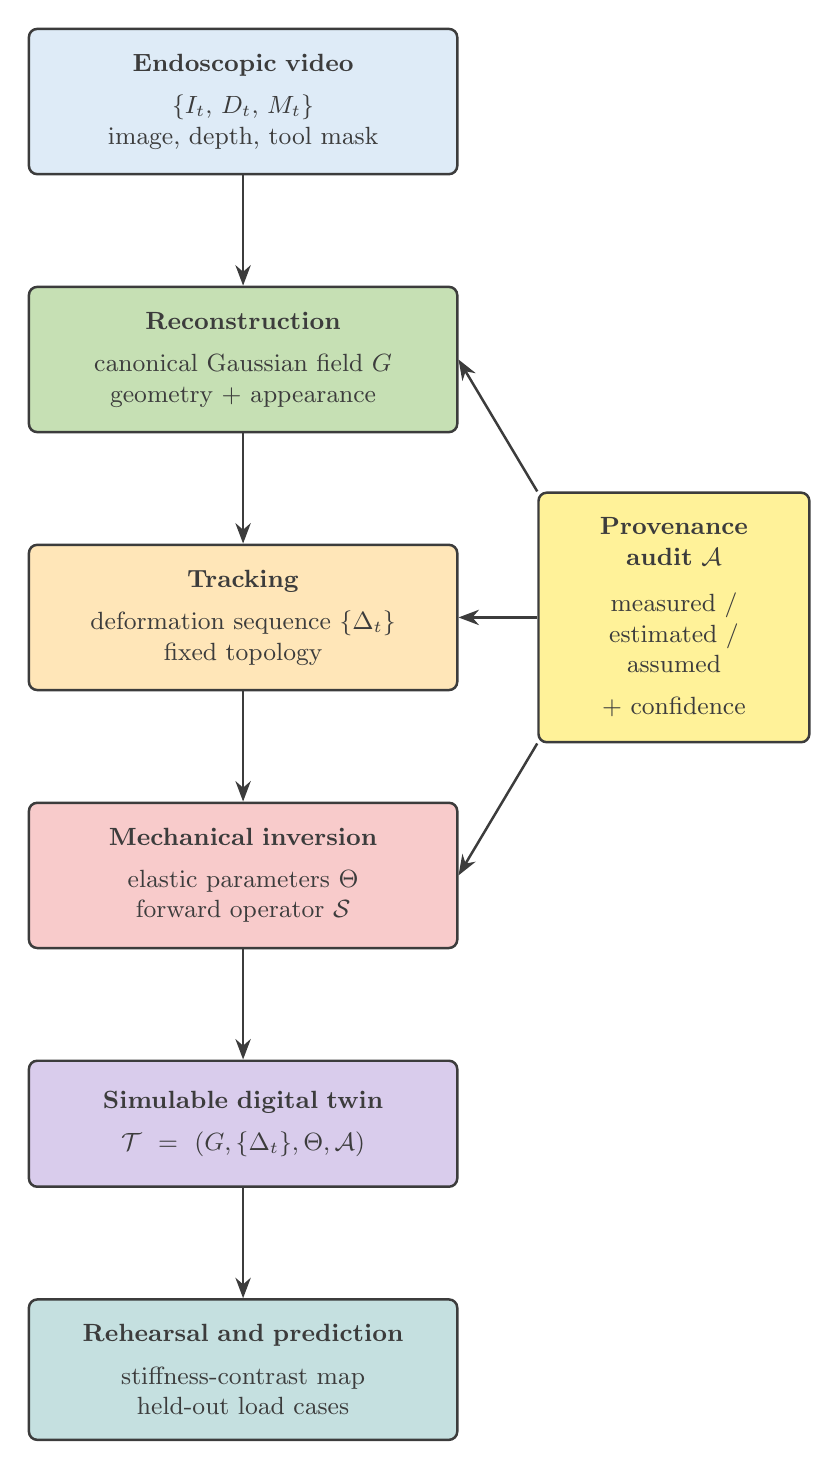
\begin{tikzpicture}[node distance=14mm]

\node[box, fill=cIn] (input)
  {\textbf{Endoscopic video}\\[1.5mm]
   $\{I_t,\, D_t,\, M_t\}$\\
   image, depth, tool mask};

\node[box, fill=cT1, below=of input] (recon)
  {\textbf{Reconstruction}\\[1.5mm]
   canonical Gaussian field $G$\\
   geometry + appearance};

\node[box, fill=cT2, below=of recon] (track)
  {\textbf{Tracking}\\[1.5mm]
   deformation sequence $\{\Delta_t\}$\\
   fixed topology};

\node[box, fill=cT3, below=of track] (inv)
  {\textbf{Mechanical inversion}\\[1.5mm]
   elastic parameters $\Theta$\\
   forward operator $\mathcal{S}$};

\node[box, fill=cTwin, below=of inv] (twin)
  {\textbf{Simulable digital twin}\\[1.5mm]
   $\mathcal{T}=(G,\{\Delta_t\},\Theta,\mathcal{A})$};

\node[box, fill=cUse, below=of twin] (use)
  {\textbf{Rehearsal and prediction}\\[1.5mm]
   stiffness-contrast map\\
   held-out load cases};

\node[audit, fill=cAudit, right=10mm of track] (audit)
  {\textbf{Provenance}\\ \textbf{audit} $\mathcal{A}$\\[2mm]
   measured /\\ estimated /\\ assumed\\[1.5mm]
   + confidence};

\draw[arr] (input) -- (recon);
\draw[arr] (recon) -- (track);
\draw[arr] (track) -- (inv);
\draw[arr] (inv) -- (twin);
\draw[arr] (twin) -- (use);

\draw[arr] (audit.west) -- (track.east);
\draw[arr] (audit.north west) -- (recon.east);
\draw[arr] (audit.south west) -- (inv.east);

\end{tikzpicture}
\end{document}
